\begin{figure}[t!]
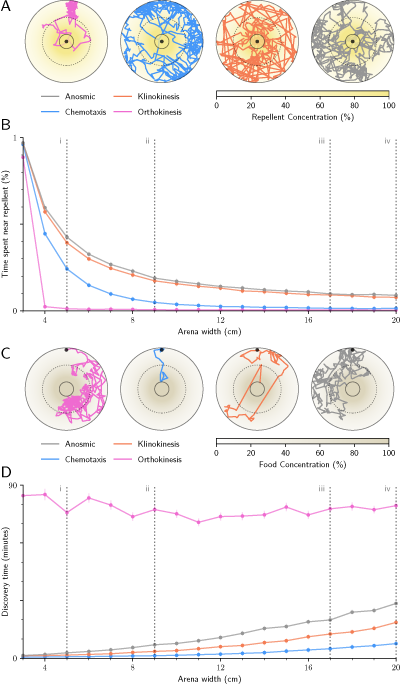
\includegraphics[width=\linewidth]{Figures/images/5.eps}
 \captionof{figure}{\textbf{Chemokinesis is superior to chemotaxis for avoiding repellents in realistic larval environments.} A: Sample trajectories for the repellent-avoidance task. B: Success of each search strategy in the repellent-avoidance task (mean ${\pm}$ standard error). C: Sample trajectories for the foraging task. (A,C): Dotted lines mark 50${\%}$ concentration. Foraging trajectories begin at the top of the 6cm-diameter arena, and repellent-avoidance task trajectories at the arena center (black dot). Starting point was randomized in actual analyses. D: Success of simulated search strategies in the foraging task. (B,D): Dashed grey lines correspond to ecologically relevant habitat sizes described in Table 2.}
 \label{fig:fig1}
\end{figure}